\documentclass[12pt, varwidth, border={5mm 5mm 5mm 5mm}]{standalone}
\usepackage{tikz}
\usepackage{amsmath}
% Underlining package
\usepackage{ulem}
\usetikzlibrary{angles,quotes}
\usetikzlibrary{intersections}
\usetikzlibrary{arrows.meta}
\usetikzlibrary{calc}
% \usepackage[a4paper, portrait, margin=1cm]{geometry}


\begin{document}
\section*{ }
    \begin{minipage}{0.75\textwidth}
  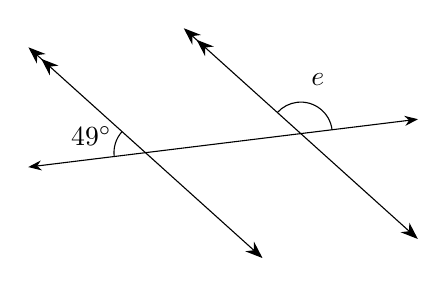
\begin{tikzpicture}[scale=1.0, baseline=(current bounding box.north)]
    \begin{scope}[rotate=7]
      % Draw the first line
      \draw[<->>, >={Stealth[scale=1.3]}, name path=P1] (0, 0) -- (-2.6242361159620287, 3.0188383208910885);
      % Draw the second line with the calculated offsets
      \draw[<->>, >={Stealth[scale=1.3]}, name path=P2] (1.9875194900232167, 0) -- (-0.636716625938812, 3.0188383208910885);
      % Draw the transversal through the middle of the parallel lines
      \draw[<->, >=Stealth, name path=P3] (-2.8121180579810146, 1.5094191604455443) -- (2.175401432042203, 1.5094191604455443);
      
      \path [name intersections={of=P1 and P3,by=A}];
      \path [name intersections={of=P2 and P3,by=B}];

      % Draw the angle
      \coordinate (p1s) at (0, 0);
      \coordinate (p1e) at (-2.6242361159620287, 3.0188383208910885);
      \coordinate (p2s) at (1.9875194900232167, 0);
      \coordinate (p2e) at (-0.636716625938812, 3.0188383208910885);
      \coordinate (ts) at (-2.8121180579810146, 1.5094191604455443);
      \coordinate (te) at (2.175401432042203, 1.5094191604455443);

      % order for vertices go in anticlockwise order te--A--p1e
      \draw pic["$e$", draw=black, -, angle eccentricity=1.8, angle radius=0.4cm] {angle=te--B--p2e};
\draw pic["$49^\circ$", draw=black, -, angle eccentricity=1.8, angle radius=0.4cm] {angle=p1e--A--ts};

      % %% Point A
      % \draw pic["$a$", draw=black, -, angle eccentricity=2.0, angle radius=0.4cm] {angle=te--A--p1e};
      % \draw pic["$b$", draw=black, -, angle eccentricity=2.0, angle radius=0.4cm] {angle=p1e--A--ts};
      % \draw pic["$c$", draw=black, -, angle eccentricity=2.0, angle radius=0.4cm] {angle=ts--A--p1s};
      % \draw pic["$d$", draw=black, -, angle eccentricity=2.0, angle radius=0.4cm] {angle=p1s--A--te};
      
      % %%  Point B
      % \draw pic["$e$", draw=black, -, angle eccentricity=2.0, angle radius=0.4cm] {angle=te--B--p2e};
      % \draw pic["$f$", draw=black, -, angle eccentricity=2.0, angle radius=0.4cm] {angle=p2e--B--ts};
      % \draw pic["$g$", draw=black, -, angle eccentricity=2.0, angle radius=0.4cm] {angle=ts--B--p2s};
      % \draw pic["$h$", draw=black, -, angle eccentricity=2.0, angle radius=0.4cm] {angle=p2s--B--te};

    \end{scope}
  \end{tikzpicture}
\end{minipage}%
\hfill
\begin{minipage}{0.2\textwidth}
  \begin{align*}
    \angle \text{e} &= \text{131}^\circ
  \end{align*}
\end{minipage}
\end{document}
